\documentclass[tikz, border=10pt]{standalone}

\usepackage{pgfplots}
% set plot's width and pgf compatibility
\pgfplotsset{width=10cm, compat=1.9}

\begin{document}
    \sffamily\bfseries
    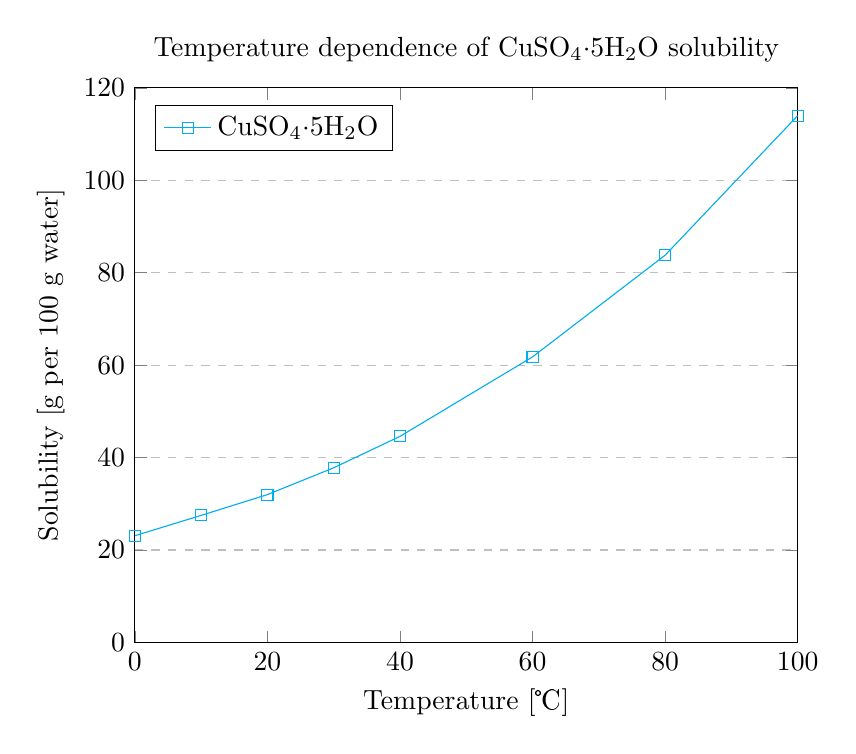
\begin{tikzpicture}
        % start drawing plot
        \begin{axis}[
            title = {Temperature dependence of CuSO\(_4\cdot\)5H\(_2\)O solubility},    % title of the plot
            xlabel = {Temperature [\textcelsius]},  % label of x axis
            ylabel = {Solubility [g per 100 g water]},  % label of y axis
            xmin = 0, xmax = 100,   % lower and upper limits of x axis
            ymin = 0, ymax = 120,   % lower and upper limits of y axis
            xtick = {0, 20, 40, 60, 80, 100},   % x sticks
            ytick = {0, 20, 40, 60, 80, 100, 120},  % y sticks
            legend pos = north west,    % where to place the plot's legend
            ymajorgrids = true,     % set horizontal grid lines
            grid style = dashed     % set grid line's style
        ]
            % plot is drawn by using coordinates
            \addplot[color=cyan, mark=square] coordinates {(0,23.1)(10,27.5)(20,32)(30,37.8)(40,44.6)(60,61.8)(80,83.8)(100,114)};
            % add legend entry
            \addlegendentry{CuSO\(_4\cdot\)5H\(_2\)O}
        \end{axis}
    \end{tikzpicture}
\end{document}